\documentclass{article}\usepackage[utf8]{inputenc}\usepackage[T1]{fontenc}\usepackage{lmodern}\usepackage{amsmath}\usepackage{tikz}\pagestyle{empty}\begin{document}\begin{center}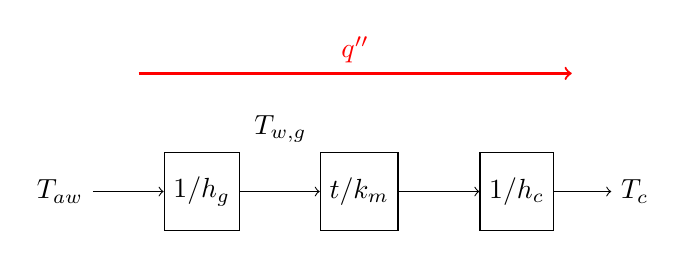
\begin{tikzpicture}\node (a) at (0,1) {$T_{aw}$};\node[draw,minimum height=1cm] (b) at (1.8,1) {$1/h_g$};\node[draw,minimum height=1cm] (c) at (3.8,1) {$t/k_m$};\node[draw,minimum height=1cm] (d) at (5.8,1) {$1/h_c$};\node (e) at (7.3,1) {$T_c$};\draw[->] (a)--(b);\draw[->] (b)--(c);\draw[->] (c)--(d);\draw[->] (d)--(e);\node at (2.8,1.8) {$T_{w,g}$};\draw[->,red,thick] (1,2.5)--(6.5,2.5) node[midway,above] {$q^{\prime\prime}$};\end{tikzpicture}\end{center}\end{document}